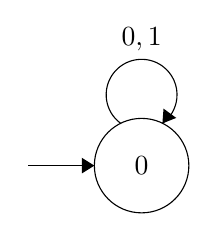
\begin{tikzpicture}[scale=0.2]
    \tikzstyle{every node}+=[inner sep=0pt]
    \draw [black] (7.4,-9) circle (3);
    \draw (7.4,-9) node {$0$};
    \draw [black] (0.2,-9) -- (4.4,-9);
    \fill [black] (4.4,-9) -- (3.6,-8.5) -- (3.6,-9.5);
    \draw [black] (6.077,-6.32) arc (234:-54:2.25);
    \draw (7.4,-1.75) node [above] {$0, 1$};
    \fill [black] (8.72,-6.32) -- (9.6,-5.97) -- (8.79,-5.38);
    \end{tikzpicture}